% Options for packages loaded elsewhere
\PassOptionsToPackage{unicode}{hyperref}
\PassOptionsToPackage{hyphens}{url}
%
\documentclass[
  10pt,
]{article}
\usepackage{amsmath,amssymb}
\usepackage{iftex}
\ifPDFTeX
  \usepackage[T1]{fontenc}
  \usepackage[utf8]{inputenc}
  \usepackage{textcomp} % provide euro and other symbols
\else % if luatex or xetex
  \usepackage{unicode-math} % this also loads fontspec
  \defaultfontfeatures{Scale=MatchLowercase}
  \defaultfontfeatures[\rmfamily]{Ligatures=TeX,Scale=1}
\fi
\usepackage{lmodern}
\ifPDFTeX\else
  % xetex/luatex font selection
\fi
% Use upquote if available, for straight quotes in verbatim environments
\IfFileExists{upquote.sty}{\usepackage{upquote}}{}
\IfFileExists{microtype.sty}{% use microtype if available
  \usepackage[]{microtype}
  \UseMicrotypeSet[protrusion]{basicmath} % disable protrusion for tt fonts
}{}
\makeatletter
\@ifundefined{KOMAClassName}{% if non-KOMA class
  \IfFileExists{parskip.sty}{%
    \usepackage{parskip}
  }{% else
    \setlength{\parindent}{0pt}
    \setlength{\parskip}{6pt plus 2pt minus 1pt}}
}{% if KOMA class
  \KOMAoptions{parskip=half}}
\makeatother
\usepackage{xcolor}
\usepackage[top=2cm,bottom=1.5cm,left=1.5cm,right=1.5cm]{geometry}
\usepackage{longtable,booktabs,array}
\usepackage{calc} % for calculating minipage widths
% Correct order of tables after \paragraph or \subparagraph
\usepackage{etoolbox}
\makeatletter
\patchcmd\longtable{\par}{\if@noskipsec\mbox{}\fi\par}{}{}
\makeatother
% Allow footnotes in longtable head/foot
\IfFileExists{footnotehyper.sty}{\usepackage{footnotehyper}}{\usepackage{footnote}}
\makesavenoteenv{longtable}
\usepackage{graphicx}
\makeatletter
\def\maxwidth{\ifdim\Gin@nat@width>\linewidth\linewidth\else\Gin@nat@width\fi}
\def\maxheight{\ifdim\Gin@nat@height>\textheight\textheight\else\Gin@nat@height\fi}
\makeatother
% Scale images if necessary, so that they will not overflow the page
% margins by default, and it is still possible to overwrite the defaults
% using explicit options in \includegraphics[width, height, ...]{}
\setkeys{Gin}{width=\maxwidth,height=\maxheight,keepaspectratio}
% Set default figure placement to htbp
\makeatletter
\def\fps@figure{htbp}
\makeatother
\setlength{\emergencystretch}{3em} % prevent overfull lines
\providecommand{\tightlist}{%
  \setlength{\itemsep}{0pt}\setlength{\parskip}{0pt}}
\setcounter{secnumdepth}{-\maxdimen} % remove section numbering
\usepackage{amsmath}
\usepackage{amssymb}
\usepackage{booktabs}
\usepackage{xcolor}
\usepackage{xfrac}
\usepackage{stackrel}
\usepackage{cancel}
\usepackage{tikz}  % per \foreach
\usepackage{layout}
\usepackage{array}
\usepackage{fancyhdr}
\pagestyle{fancy}
\usepackage{comment}
\usepackage{fancyhdr}
\usepackage{float}

\usepackage{color}
\usepackage{colortbl}
\usepackage{multirow}


% solo shiny
\usepackage{draftwatermark}
\SetWatermarkText{FAC-SIMILE}
\SetWatermarkScale{1}
\SetWatermarkColor[gray]{0.95}
\SetWatermarkAngle{45}
% fine solo shiny


\pagestyle{fancy} % Imposta lo stile fancy come predefinito

% Definisci uno stile di pagina senza numeri
\fancypagestyle{senzanumero}{%
  \fancyhf{} % Pulisce intestazione e piè di pagina
}


\fancyhf{}
\lhead{\textbf{Compito di Statistica (CLEAM)}}
\cfoot{\thepage}
\usepackage{etoolbox}
\excludecomment{sol} 
\definecolor{mygray}{gray}{0.6}

%\pagestyle{empty}

\newcommand{\quadratini}[1]{%
  \foreach \i in {1,...,#1}{%
    \fcolorbox{mygray}{white}{\phantom{\huge A}}%
    \hspace{0.5em}%
  }%
}

\newcommand{\anagrafica}{%
 % \vspace{-14cm}
  {\sffamily % font sans-serif attivo
  {Compilare in Stampatello}\\[0.5em]
  \begin{tabular}{>{\sffamily}r l}
    COGNOME: & \quadratini{18} \\[0.5em]
    NOME: & \quadratini{18} \\[0.5em]
    Matricola: & \quadratini{8} \\[0.5em]
    %Codice: & \texttt{#1} \\
  \end{tabular}\\
  \vspace{-.5cm}
  \noindent\rule{\textwidth}{0.4pt}
  } % chiusura \sffamily
}
\ifLuaTeX
  \usepackage{selnolig}  % disable illegal ligatures
\fi
\usepackage{bookmark}
\IfFileExists{xurl.sty}{\usepackage{xurl}}{} % add URL line breaks if available
\urlstyle{same}
\hypersetup{
  hidelinks,
  pdfcreator={LaTeX via pandoc}}

\author{}
\date{\vspace{-2.5em}}

\begin{document}

\vspace*{-1.4cm}
\anagrafica{}

\thispagestyle{fancy}
\fancypagestyle{firstpage}{%
  \lhead{\textbf{Prova di Statistica (CLEAM)}}
  \rhead{\texttt{S0CD48MFPA9QNZI}}
  \cfoot{} % Rimuove il numero di pagina
}
\pagestyle{firstpage}

\subsubsection{Esercizio 1}\label{esercizio-1}

Su un campione di \(160\) famiglie dell'Emilia-Romagna sono stati rilevati i consumi annui in beni tecnologici (dai espressi in migliaia di euro). Qui di seguito la distribuzione delle densità percentuali:

\begin{table}[H]
\centering
\begin{tabular}{rrr}
\toprule
$[\text{x}_j,$ & $\text{x}_{j+1})$ & $h_j$\\
\midrule
0.0 & 1.5 & 12.0833\\
1.5 & 3.0 & 23.7500\\
3.0 & 8.0 & 7.8750\\
8.0 & 20.0 & 0.5729\\
 &  & \\
\bottomrule
\end{tabular}
\end{table}

1.a (pt\hspace{.1em}3.9/31) Calcolare il valore approssimativo della mediana.

\begin{sol}

\begin{eqnarray*}
  p &=&  0.5 , \text{essendo }F_{ 2 }= 0.5375  > 0.5  \Rightarrow j_{ 0.5 }= 2 \\
  x_{ 0.5 } &=& x_{\text{inf}; 2 } + \frac{ { 0.5 } - F_{ 1 }} {f_{ 2 }} \cdot b_{ 2 } \\
            &=&  1.5  + \frac {{ 0.5 } -  0.1812 } { 0.3563 } \cdot  1.5  \\
            &=&  2.842 
\end{eqnarray*}

\begin{center}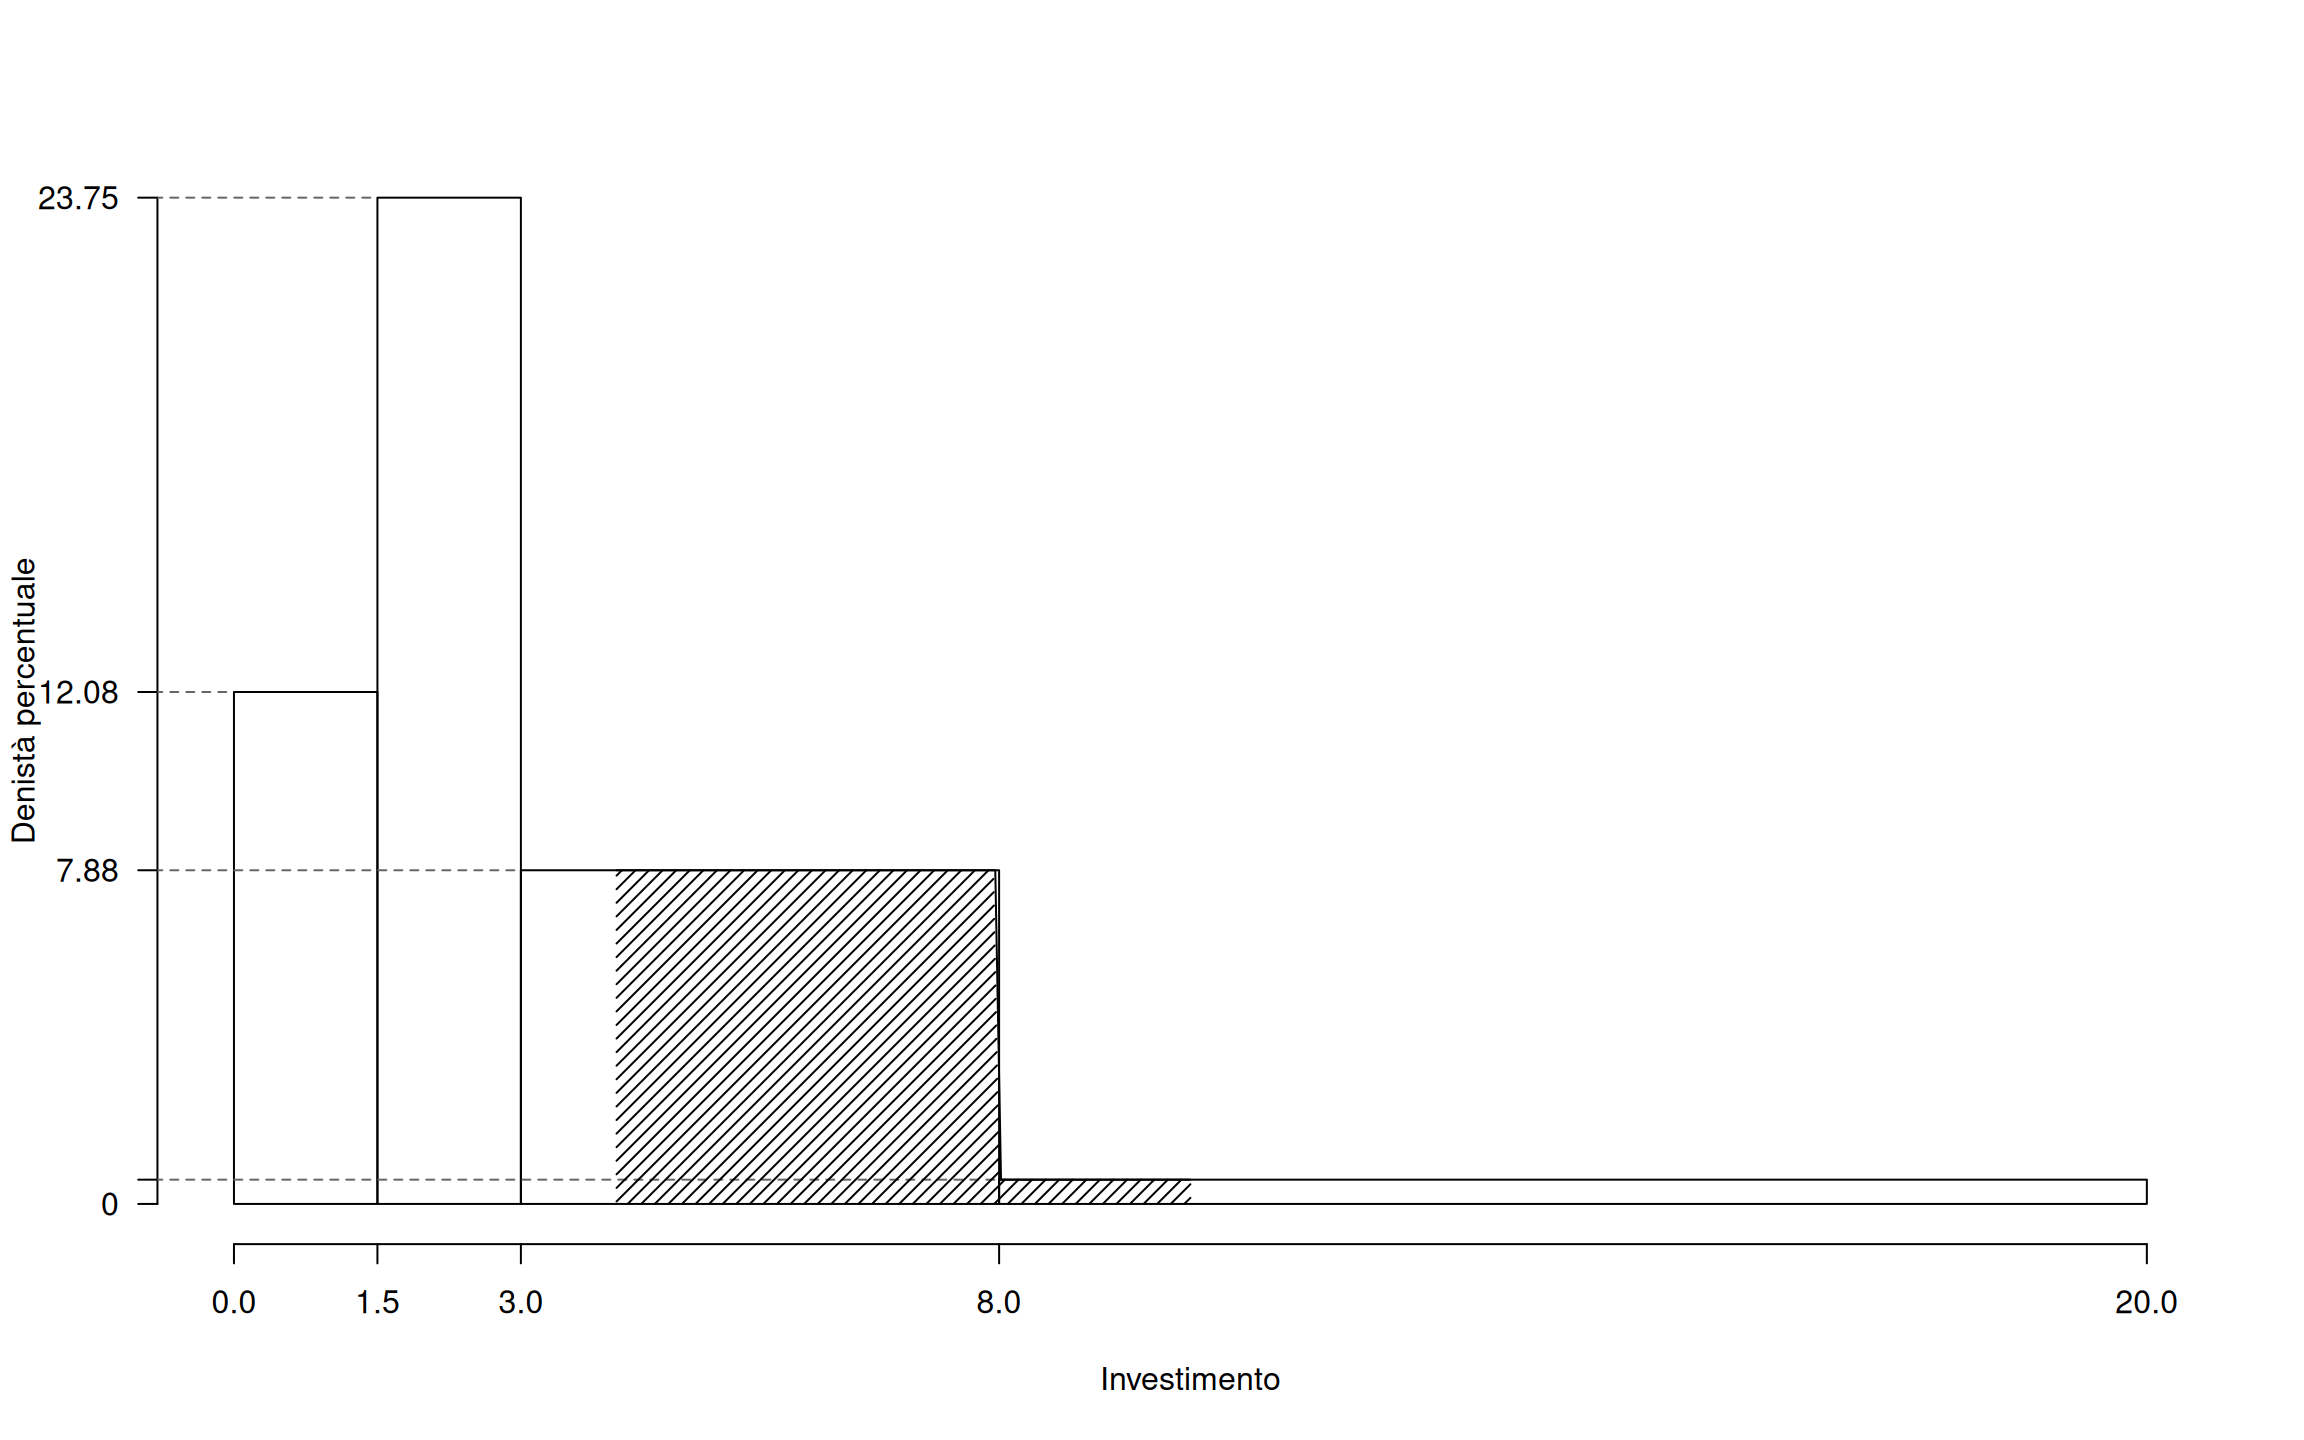
\includegraphics{www/compito_files/figure-latex/2024-95-1} \end{center}

\end{sol}

1.b (pt\hspace{.1em}1.2/31) Qual è la percentuale di famiglie spendono più del 55-esimo percentile \(x_{0.55}\)?

\begin{sol}
Per definizione \(\%(X>x_{0.55})=45\%\) e
\(\#(X>x_{0.55})\approx0.45\times160 =72\)

\end{sol}

1.c (pt\hspace{.1em}0.6/31) La media è pari a \(\bar x=4\), senza disegnare l'istogramma, che forma distributiva dobbiamo aspettarci?

1.d (pt\hspace{.1em}0.6/31) La spesa media è pari a \(4.0009\), mentre la varianza è pari a \(10.6517\).
Se ogni famiglia diminuisse la propria spesa del 2\%, quanto varrebbero la media e la varianza dei dati così trasformati?

\begin{sol}
\[
\bar y = 3.9209\qquad \sigma^2 = 10.2299
\]

\end{sol}

\subsubsection{Esercizio 2}\label{esercizio-2}

2.a (pt\hspace{.1em}3.9/31) Si consideri un'urna che ha 5 palline bianche, 5 nere e 5 verdi. Si estrae 3 volte \textbf{con} reinserimento. Sia \(X\) la variabile casuale che conta il numero di bianche su 3 estrazioni. Calcolare la probabilità che \(X\leq 1\).

\begin{sol}
\normalsize 
\begin{eqnarray*}
      P( X \leq 1 ) &=& \binom{ 3 }{ 0 } 0.3333 ^{ 0 }(1- 0.3333 )^{ 3 - 0 }+\binom{ 3 }{ 1 } 0.3333 ^{ 1 }(1- 0.3333 )^{ 3 - 1 } \\                 &=& 0.2963+0.4444 \\                 &=& 0.7407 
   \end{eqnarray*}
\normalsize 

\end{sol}

2.b (pt\hspace{.1em}1.2/31) Si consideri un'urna che ha 5 palline bianche, 5 nere e 5 verdi. Si estrae 3 volte \textbf{senza} reinserimento. Sia \(X\) la variabile casuale che conta il numero di bianche su 3 estrazioni. Calcolare la probabilità che \(X\leq 1\).

\begin{sol}
\begin{eqnarray*}
  B_i &=& \text{Bianca all'estrazione $i$}\\
  \bar B_i &=& \text{Non Bianca all'estrazione $i$}\\
  P(X\le 1) &=&  P(X=0) + P(X=1)\\
   &=& P(\bar B_1\cap\bar B_2\cap\bar B_3)+\\
   &+&P(B_1\cap\bar B_2 \cap \bar B_3)+P(\bar B_1\cap B_2 \cap \bar B_3)+P(\bar B_1\cap\bar B_2 \cap B_3)\\
   &=& \frac {10}{15}\frac {9}{14}\frac {8}{13}+3\cdot\frac {5}{15}\frac {10}{14}\frac {9}{13}\\
  &=& 0.3956
\end{eqnarray*}

\end{sol}

2.c (pt\hspace{.1em}0.6/31) Sia \(X\) una VC definita su \(S_X=\{0,1,2,3\}\), posto \(Y=2X\) ricavare \(S_Y\).

2.d (pt\hspace{.1em}0.6/31) Sia \(X\) una VC, e siano \(P(X\leq 1)=0.1\), \(P(X> 2)=0.1\). Calcolare
\[
P(X>2|X>1)
\]

\begin{sol}
\begin{eqnarray}
  P(X>2|X>1) &=&  \frac{P({X>2}\cap {X>1})}{P(X> 1)}\\
             &=&  \frac{P({X>2})}{P(X> 1)}\\
             &=&   \frac{0.1}{1-0.1}\\
             &=& 0.1111
\end{eqnarray}

\end{sol}

\subsubsection{Esercizio 3}\label{esercizio-3}

3.a (pt\hspace{.1em}3.9/31) Un'urna contiene 2 palline numerate con \(\fbox{0}\), 6 numerate con \(\fbox{1}\) e 2 numerate con \(\fbox{2}\). Si estrae 100 volte con reinserimento. Qual è la probabilità che la proporzione di palline col numero \(\fbox{1}\) sia minore di 0.55?

\begin{sol}
\[
\pi = P(\text{estrarre $\fbox{1}$})=\frac {6}{10}=0.6
\]
\textbf{Teorema del Limite Centrale (proporzione)}

Siano \(X_1\),\ldots,\(X_n\), \(n=100\) VC IID, tc \(X_i\sim\text{Ber}(\pi=0.6)\)\(,\forall i\), posto:
\[
      \hat\pi=\frac{S_n}n = \frac{X_1 + ... + X_n}n
      \]
allora:\begin{eqnarray*}
  \hat\pi & \mathop{\sim}\limits_{a}& N(\pi,\pi(1-\pi)/n) \\
  &\sim & N\left(0.6,\frac{0.6\cdot(1-0.6)}{100}\right) \\
     &\sim & N(0.6,0.0024) 
  \end{eqnarray*}\begin{eqnarray*}
      P( \hat\pi   <   0.55 ) 
        &=& P\left(  \frac { \hat\pi  -  \pi }{ \sqrt{\pi(1-\pi)/n} }  <  \frac { 0.55  -  0.6 }{\sqrt{ 0.0024 }} \right)  \\
                 &=& P\left(  Z   <   -1.02 \right) \\    
                 &=&  1-\Phi( 1.02 ) \\ &=&  0.1539 
      \end{eqnarray*}

\end{sol}

\subsubsection{Esercizio 4}\label{esercizio-4}

4.a (pt\hspace{.1em}0.9/31) Siano \(h_1\) e \(h_2\) due stimatori per \(\theta\), tali che

\[
  MSE(h_1) =  \frac{\theta}{n^2}, \qquad  MSE(h_2) =  \frac{\theta}{n}
\]

Quale dei due stimatori è più efficiente?

4.b (pt\hspace{.1em}0.9/31) Siano \(T_1\) e \(T_2\) due test statistici per la stessa \(H_0\) e con la stessa significatività \(\alpha\). Cosa significa dire che \(T_1\) e più potente di \(T_2\)?

4.c (pt\hspace{.1em}0.9/31) Definire la probabilità di significatività osservata.

4.d (pt\hspace{.1em}0.9/31) Se in un test statistico che utilizza la statistica test \emph{t} con 10 gradi di libertà \(t_\text{obs}=1.4\), il \(p_\text{value}\) sarà maggiore o minore di 0.05? Perché?

\subsubsection{Esercizio 5}\label{esercizio-5}

Nel comune \(A\) si è condotta un'intervista per conoscere l'opinione
dei cittadini sulla presenza di un inceneritore. Sono state intervistate
25 persone a cui è stato chiesto di esprimete l'opinione in una scala da zero a 100.
È risultato un punteggio medio pari a \(\hat\mu_A=72.1\) con una standard deviation
\(\hat\sigma_A=3.4\)

5.a (pt\hspace{.1em}0.9/31) Costruire un intervallo di confidenza al 95\%
per la proporzione dei favorevoli in popolazione.

\begin{sol}
\(1-\alpha =0.95\) e quindi \(\alpha=0.05\rightarrow \alpha/2=0.025\)

\[
      S  =\sqrt{\frac {n}{n-1}}\cdot\hat\sigma =
     \sqrt{\frac { 25 }{ 24 }}\cdot 3.4 = 3.4701 
\]
\begin{eqnarray*}
  Idc: & &  \hat\mu \pm  t_{n-1;\alpha/2} \times \frac{S}{\sqrt{n}} \\
     & &  72.1 \pm  2.064 \times \frac{ 3.4701 }{\sqrt{ 25 }} \\
     & &  72.1 \pm  2.064 \times  0.694 \\
     & & [ 70.67 ,  73.53 ]
\end{eqnarray*}

\end{sol}

5.b (pt\hspace{.1em}3.0/31) Nel comune \(B\) si è condotta un'intervista analoga.
Sono state intervistate 23 persone si è osservata una media pari \(\mu_B=69.6\) e una deviazione standard \(\hat\sigma_B=3.3\).
Sotto ipotesi di omogeneità testare l'ipotesi che le medie dei due comuni siano uguali contro l'alternativa che siano diverse

\begin{sol}
\textbf{Test \(T\) per due medie, (omogeneità)}

\(\fbox{A}\) FORMULAZIONE DELLE IPOTESI

\[\begin{cases}
   H_0: \mu_\text{A} = \mu_\text{B} \\
   H_1: \mu_\text{A} \neq \mu_\text{B} 
   \end{cases}\]

\(\fbox{B}\) SCELTA E CALCOLO STATISTICA-TEST, \(T\)

L'ipotesi è di omogeneità e quindi calcoliamo:\[
   S_p^2=\frac{n_\text{ A }\hat\sigma^2_\text{ A }+n_\text{ B }\hat\sigma^2_\text{ B }}{n_\text{ A }+n_\text{ B }-2} =
   \frac{ 25 \cdot 3.4 ^2+ 24 \cdot 3.3 ^2}{ 25 + 24 -2}= 11.71 
  \]

\begin{eqnarray*}
  \frac{\hat\mu_\text{ A } - \hat\mu_\text{ B }}
  {\sqrt{\frac {S^2_p}{n_\text{ A }}+\frac {S^2_p}{n_\text{ B }}}}&\sim&t_{n_\text{ A }+n_\text{ B }-2}\\
  t_{\text{obs}}
  &=& \frac{ ( 72.1 -  69.6 )} {\sqrt{\frac{ 11.71 }{ 25 }+\frac{ 11.71 }{ 24 }}}
  =   2.556 \, .
  \end{eqnarray*}

\(\fbox{C}\) CONCLUSIONE

Siccome \(H_1\) è bilaterale, considereremo \(\alpha/2\),
anziché \(\alpha\)

\(\alpha=0.1, 0.05, 0.01, 0.001\) e quindi \(\alpha/2=0.05, 0.025, 0.005, 0.0005\)

I valori critici sono

\(t_{49-2;0.05}=1.6779\); \(t_{49-2;0.025}=2.0117\); \(t_{49-2;0.005}=2.6846\); \(t_{49-2;0.0005}=3.5099\)

Siccome \(2.0117<|t_\text{obs}|=2.5565<2.6846\), quindi \textbf{rifiuto} \(H_0\) al 5\%,

\(0.01<p_\text{value}<0.05\), \emph{significativo} \(\fbox{*}\).

\begin{center}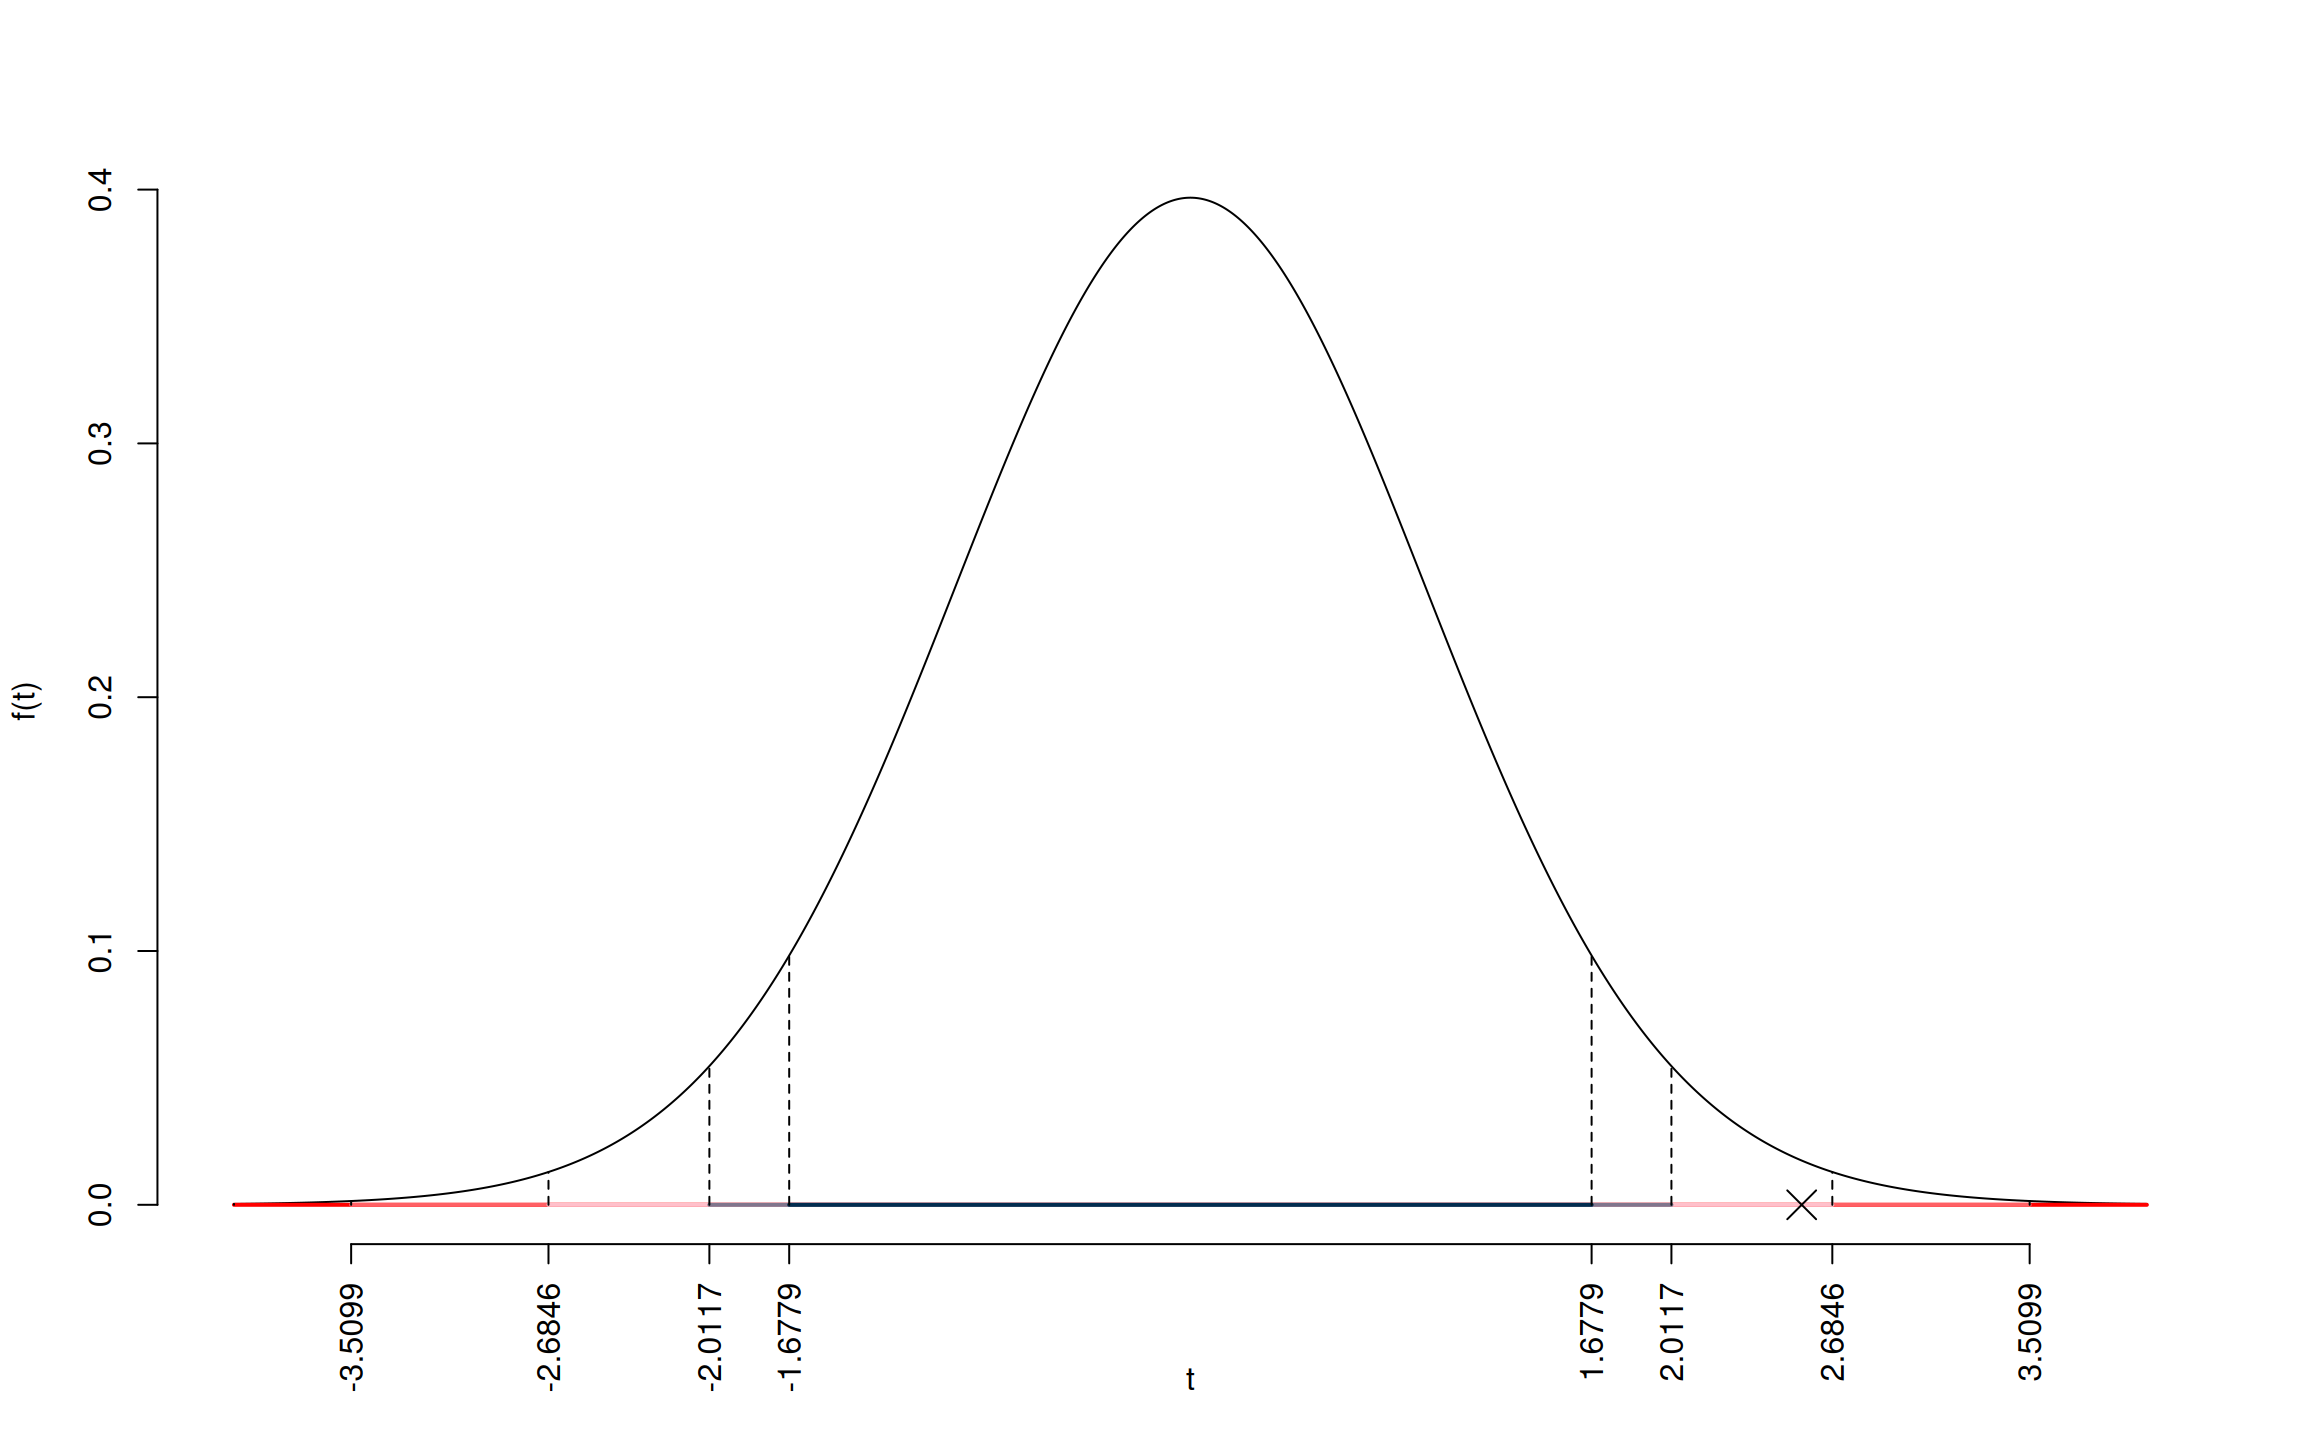
\includegraphics{www/compito_files/figure-latex/2023-71,-1} \end{center}

Il \(p_{\text{value}}\) è

\[ p_{\text{value}} = P(|T_{49-2}|>|2.56|)=2P(T_{49-2}>2.56)=0.013864 \]

Attenzione il calcolo del \(p_\text{value}\) con la \(T\) è puramente illustrativo e non può essere riprodotto senza una calcolatrice statistica adeguata.\[
 0.01 < p_\text{value}= 0.013864 \leq 0.05 
\]

\end{sol}

\subsubsection{Esercizio 6}\label{esercizio-6}

Sono stati analizzati 15 comuni della provincia di Bologna e su ogni comune è stato rilevato
il PIL pro capite del comune \(X\), espresso in decine di migliaia di euro e un valore di percezione di
qualità della vita \(Y\) (espresso su opportuna scala).

Qui di seguito le statistiche bivariate

\begin{align*}
  \sum_{i=1}^n x_i &= 29.3 &\sum_{i=1}^n x_i^2 &= 74.51 &\sum_{i=1}^n x_i y_i &= 242.81\\
  \sum_{i=1}^n y_i &= 110.8 & \sum_{i=1}^n y_i^2 &= 866.02 &
\end{align*}

6.a (pt\hspace{.1em}3.9/31) Stimare la previsione per \(x=1.6\) nel modello di regressione dove \(Y\) viene spiegata da \(X\).

\begin{sol}
\begin{eqnarray*}
           \bar x &=&\frac 1 n\sum_{i=1}^n x_i = \frac {1}{ 15 }  29.3 =  1.953 \\
           \bar y &=&\frac 1 n\sum_{i=1}^n y_i = \frac {1}{ 15 }  110.8 =  7.387 \\
           \hat\sigma_X^2&=&\frac 1 n\sum_{i=1}^n x_i^2-\bar x^2=\frac {1}{ 15 }  74.51  - 1.9533 ^2= 1.152 \\
           \hat\sigma_Y^2&=&\frac 1 n\sum_{i=1}^n y_i^2-\bar y^2=\frac {1}{ 15 }  866  - 7.3867 ^2= 3.172 \\
           \text{cov}(X,Y)&=&\frac 1 n\sum_{i=1}^n x_i~y_i-\bar x\bar y=\frac {1}{ 15 }  242.8 - 1.9533 \cdot 7.3867 = 1.759 \\
           \hat\beta_1 &=& \frac{\text{cov}(X,Y)}{\hat\sigma_X^2} \\
                    &=& \frac{ 1.759 }{ 1.152 }  =  1.527 \\
           \hat\beta_0 &=& \bar y - \hat\beta_1 \bar x\\
                    &=&  7.387 - 1.5269 \times  1.9533 = 4.404 
         \end{eqnarray*}\[\hat y_{X= 1.6 }=\hat\beta_0+\hat\beta_1 x= 4.404 + 1.5269 \times 1.6 = 6.847 \]

\end{sol}

6.b (pt\hspace{.1em}1.2/31) Calcolare numericamente \(RSS\):
\[
RSS=\sum_{i=1}^n \hat\epsilon_i^2
\]

\begin{sol}
\[RSS=n(1-r^2)\hat\sigma_Y^2=7.2968\]

\end{sol}

6.c (pt\hspace{.1em}0.6/31) Gli stimatori \(\hat\beta_0\) e \(\hat\beta_1\) sono consistenti?
Perché?

6.d (pt\hspace{.1em}0.6/31) Se in un modello di regressione con 11 dati,
il residuo studentizzato del dato \(i\) è \(\tilde \epsilon_i=1.23\), cosa possiamo concludere?

6.e (pt\hspace{.1em}0.6/31) Sia \(\hat\beta_1\) lo stimatore dei minimi quadrati per \(\beta_1\).
Scrivere il suo Standard Error teorico.

\end{document}
